\chapter{Cambios que no tienen vuelta atrás}\label{ch:g5:irreversible-changes}

Se casca un huevo en una sartén caliente. En unos segundos, la clara
transparente y líquida se vuelve firme y blanca, y la yema se espesa.
Aparta la sartén del fuego, deja que el huevo se enfríe, mételo en la
nevera: nunca volverá a ser un huevo crudo. Algunos cambios se pueden
deshacer y otros no. Distinguirlos es el primer paso de la química.

\begin{recall}
Un sólido que se \omterm{def:g2:mixing-and-dissolving:dissolve}{disuelve} en agua sigue ahí: cuando el agua se seca, el
sólido se queda (\cref{ch:g2:mixing-and-dissolving}). Una \omterm{def:g4:what-a-fire-needs:burning}{combustión}
produce sustancias nuevas (ceniza, humo, dióxido de carbono, vapor de
agua) y el \omterm{def:g4:what-a-fire-needs:fuel}{combustible} desaparece para siempre (\cref{ch:g4:what-a-fire-needs}).
\end{recall}

\begin{omfigure}
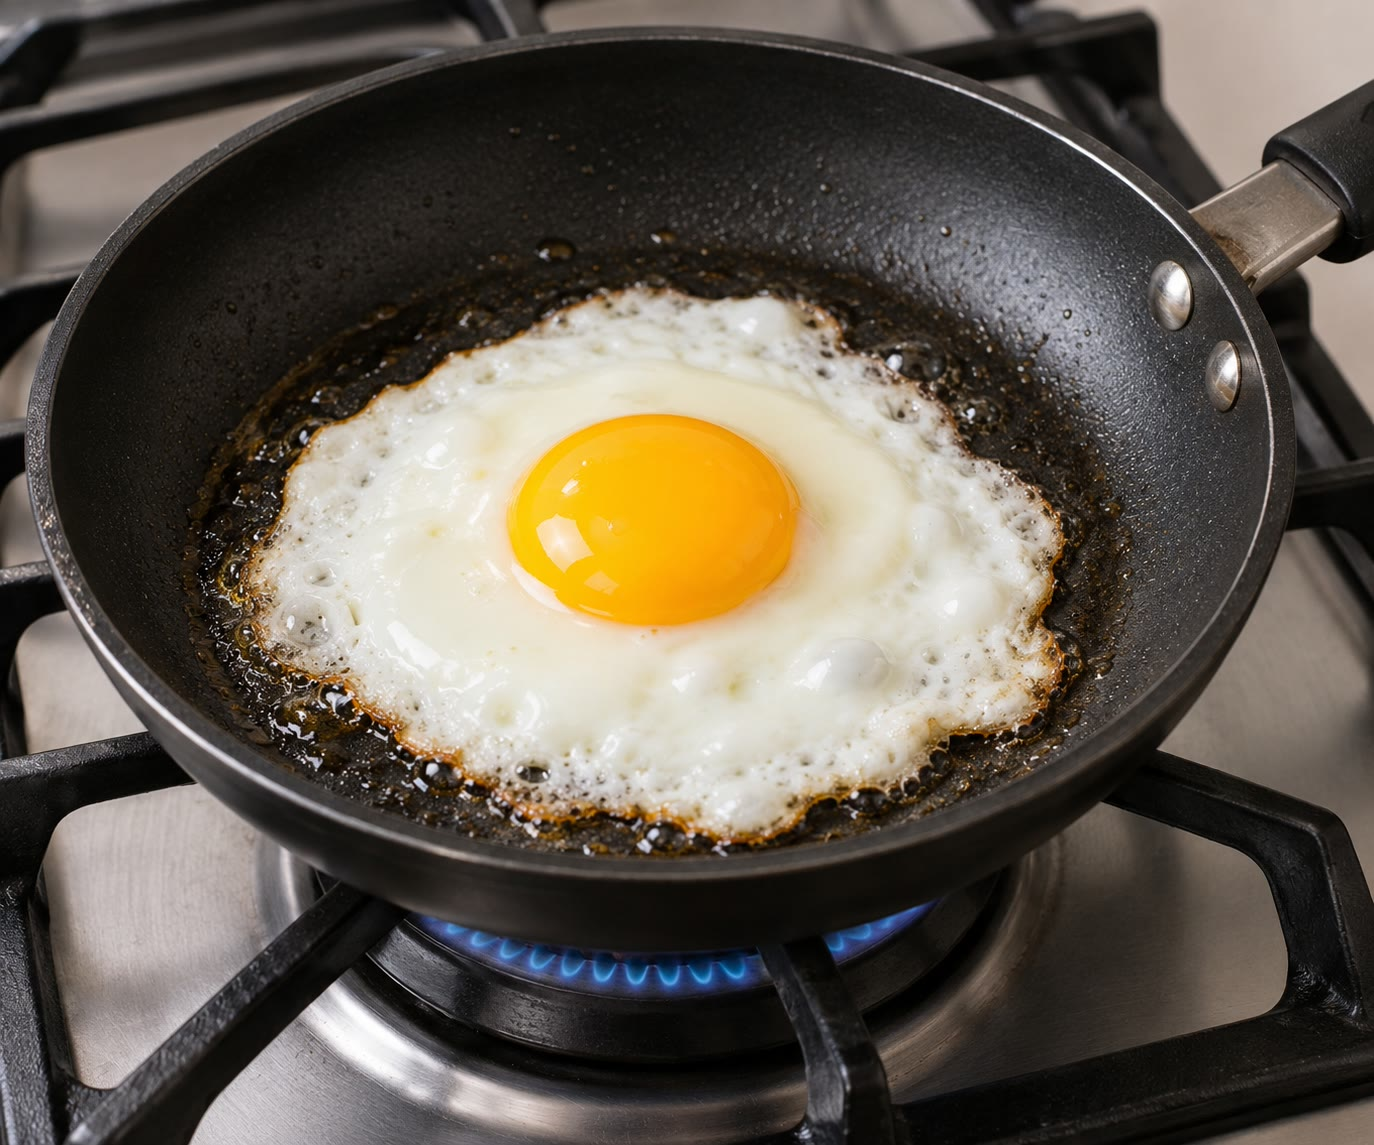
\includegraphics[width=0.55\linewidth]{images/book1/ai/g5-egg-frying.jpg}

{\small Un huevo friéndose: la clara transparente se ha vuelto firme y
blanca, para siempre.}
\end{omfigure}

\section{Cambios que se pueden deshacer}

\begin{definition}[Cambio reversible]\label{def:g5:irreversible-changes:reversible}
Un \emph{cambio reversible}\index{cambio reversible} es un cambio que se
puede deshacer, de modo que recuperamos exactamente lo que teníamos al
principio.
\end{definition}

\begin{example}[Disolver y secar]\label{ex:g5:irreversible-changes:dissolve}
El azúcar removido en agua se \omterm{def:g2:mixing-and-dissolving:dissolve}{disuelve}. Si dejamos que el agua se
evapore, el azúcar vuelve: el mismo azúcar, igual de dulce que antes.
\omterm{def:g2:mixing-and-dissolving:dissolve}{Disolver} es un \omterm{def:g5:irreversible-changes:reversible}{cambio reversible}.
\end{example}

\begin{example}[Hielo y agua]\label{ex:g5:irreversible-changes:ice}
Un cubito de hielo se funde y se convierte en agua sobre un plato
templado; si metemos el agua en el congelador, vuelve a ser hielo.
Fundirse y congelarse son \omterm{def:g5:irreversible-changes:reversible}{cambios reversibles}. (Por qué el agua se
funde y se congela lo cuenta el libro de física.)
\end{example}

\begin{example}[Mezclar]\label{ex:g5:irreversible-changes:mix}
La arena \omterm{def:g2:mixing-and-dissolving:mix}{mezclada} con grava se puede volver a separar con un tamiz; el
agua turbia se puede filtrar. \omterm{def:g2:mixing-and-dissolving:mix}{Mezclar} es un \omterm{def:g5:irreversible-changes:reversible}{cambio reversible}: no se
fabrica nada nuevo, y las partes se pueden separar
(\cref{ch:g3:separating-mixtures}).
\end{example}

\section{Cambios que no se pueden deshacer}

\begin{definition}[Cambio irreversible y cambio químico]\label{def:g5:irreversible-changes:chemical-change}
Un \emph{cambio irreversible}\index{cambio irreversible} es un cambio
que no se puede deshacer sin más. La mayoría son cambios en los que
aparecen sustancias nuevas que al principio no estaban: un cambio así se
llama \emph{cambio químico}\index{cambio quimico@cambio químico}.
\end{definition}

\begin{example}[Seis cambios químicos]\label{ex:g5:irreversible-changes:six}
\begin{itemize}
  \item \textbf{Cocinar un huevo}: la clara líquida y transparente se
        vuelve firme y blanca.
  \item \textbf{Hornear un bizcocho}: una masa líquida se convierte en
        un bizcocho esponjoso, dorado por fuera, con un olor nuevo.
  \item \textbf{\omterm{def:g4:what-a-fire-needs:burning}{Arder}}: la madera se convierte en ceniza, humo, dióxido
        de carbono y vapor de agua.
  \item \textbf{Oxidarse}: el hierro brillante que se deja bajo la
        lluvia se cubre de una sustancia anaranjada y escamosa, la
        herrumbre.
  \item \textbf{Agriarse la leche}: olvidada durante días, la leche se
        espesa, forma grumos y huele agria.
  \item \textbf{Ponerse marrón una manzana cortada}: su pulpa clara se
        vuelve marrón al \omterm{def:g4:air-a-mixture-of-gases:air}{aire} en menos de una hora.
\end{itemize}
En cada caso se ha fabricado algo nuevo, y no hay ninguna forma sencilla
de recuperar lo que teníamos al principio.
\end{example}

\begin{omfigure}
\begin{minipage}[t]{0.48\linewidth}\centering
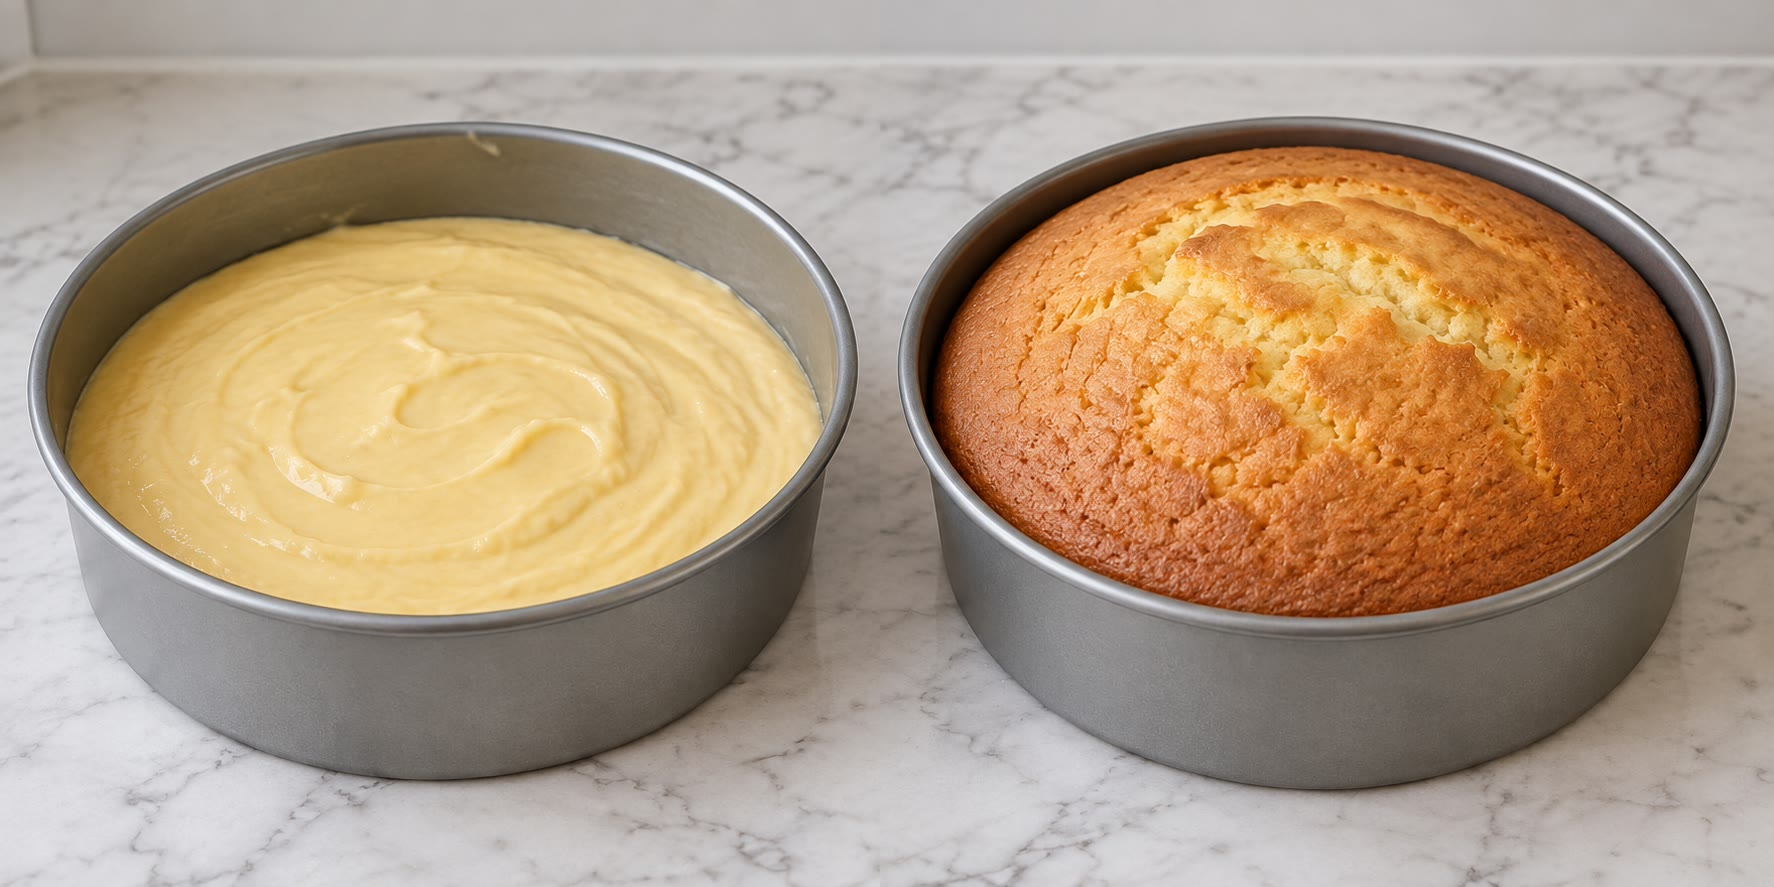
\includegraphics[width=\linewidth,height=4.6cm,keepaspectratio]{images/book1/ai/g5-cake-before-after.jpg}

{\small Masa antes, bizcocho después: hornear no tiene vuelta atrás.}
\end{minipage}\hfill
\begin{minipage}[t]{0.48\linewidth}\centering
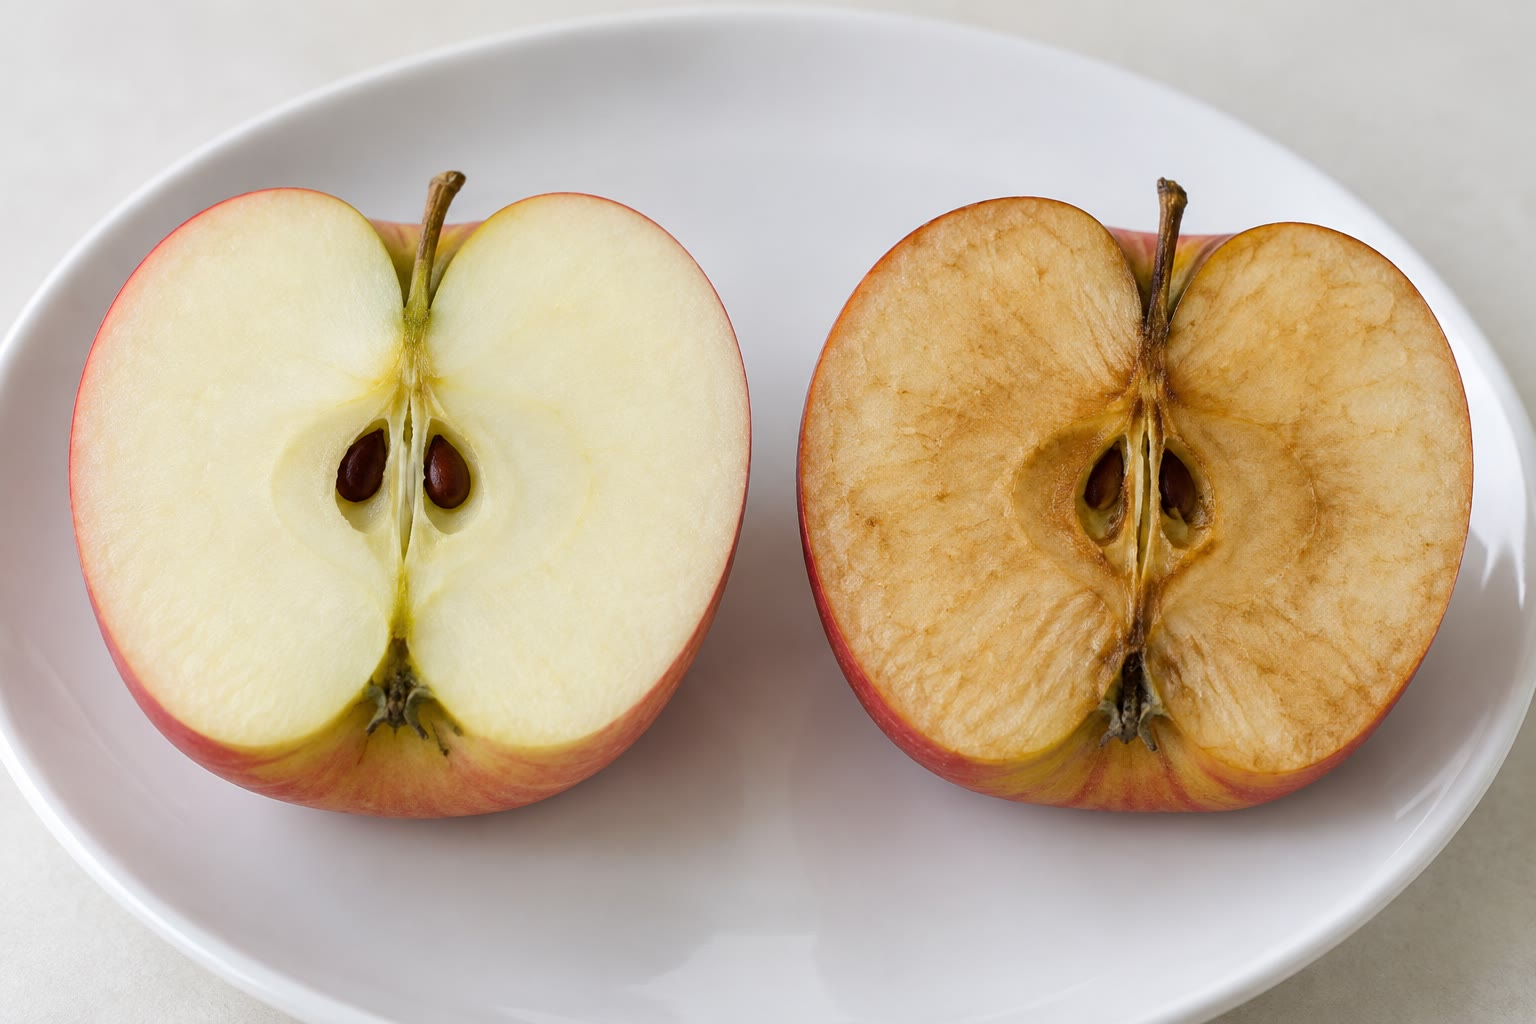
\includegraphics[width=\linewidth,height=4.6cm,keepaspectratio]{images/book1/ai/g5-apple-browning.jpg}

{\small Una mitad recién cortada y otra mitad que ha pasado una hora al
\omterm{def:g4:air-a-mixture-of-gases:air}{aire}.}
\end{minipage}
\end{omfigure}

\begin{omfigure}
\begin{tikzpicture}[font=\small]
  \node[font=\small\bfseries, omDef] at (2.7,4.6) {se puede deshacer};
  \node[font=\small\bfseries, omProp] at (9.6,4.6) {no se puede deshacer};
  \draw[black!30] (6.1,4.9) -- (6.1,-0.3);
  % reversible pairs
  \foreach \y/\a/\b in {3.6/{azúcar + agua}/{agua con azúcar}, 2.0/{hielo}/{agua líquida},
                        0.4/{arena + grava}/{una mezcla}} {
    \node[draw=omDef, fill=omDef!6, rounded corners=2pt, minimum width=2.3cm,
      minimum height=0.8cm] at (0.9,\y) {\a};
    \node[draw=omDef, fill=omDef!6, rounded corners=2pt, minimum width=2.3cm,
      minimum height=0.8cm] at (4.6,\y) {\b};
    \draw[->, thick, omDef] (2.3,\y+0.12) -- (3.25,\y+0.12);
    \draw[<-, thick, omDef] (2.3,\y-0.12) -- (3.25,\y-0.12);
  }
  % irreversible ones
  \foreach \y/\a/\b in {3.6/{huevo crudo}/{huevo cocinado}, 2.0/{madera}/{ceniza, humo, gases},
                        0.4/{hierro}/{herrumbre}} {
    \node[draw=omProp, fill=omProp!6, rounded corners=2pt, minimum width=2.0cm,
      minimum height=0.8cm] at (7.6,\y) {\a};
    \node[draw=omProp, fill=omProp!6, rounded corners=2pt, minimum width=2.9cm,
      minimum height=0.8cm] at (11.5,\y) {\b};
    \draw[->, thick, omProp] (8.8,\y) -- (9.85,\y);
  }
\end{tikzpicture}

{\small A la izquierda, \omterm{def:g5:irreversible-changes:reversible}{cambios reversibles}: la doble flecha indica que
pueden ir en los dos sentidos. A la derecha, \omterm{def:g5:irreversible-changes:chemical-change}{cambios químicos}: en un
solo sentido.}
\end{omfigure}

\section{Pistas de que ha aparecido una sustancia nueva}

\begin{method}[¿Es un cambio químico? Busca las pistas]\label{met:g5:irreversible-changes:clues}
Una sustancia nueva suele delatarse por alguna de estas pistas:
\begin{enumerate}
  \item un \textbf{color} nuevo (el dorado de una rebanada de pan
        tostado);
  \item \textbf{burbujas} de un gas que aparecen en un líquido sin
        calentarlo (vinagre vertido sobre bicarbonato);
  \item un \textbf{olor} nuevo (leche agria, tostada quemada);
  \item se desprende \textbf{calor o luz} (una vela que \omterm{def:g4:what-a-fire-needs:burning}{arde});
  \item \textbf{aparece un sólido} en un líquido transparente, o se
        forman grumos (la leche que se corta).
\end{enumerate}
Una sola pista puede engañar: el agua hirviendo burbujea, pero no se
fabrica nada nuevo; las burbujas son vapor de agua, y el agua vuelve
cuando el vapor se enfría. Busca varias pistas y pregúntate: ¿se puede
deshacer?
\end{method}

\begin{omfigure}
\begin{tikzpicture}[font=\small]
  \foreach \k/\t in {0/{color nuevo}, 1/{burbujas de gas}, 2/{olor nuevo},
                     3/{calor o luz}, 4/{aparece un sólido}} {
    \begin{scope}[xshift=\k*3.2cm]
      \draw[omProp, line width=0.8pt, fill=omProp!5] (0,0) circle (1.0);
      \node[anchor=north, align=center] at (0,-1.15) {\t};
    \end{scope}
  }
  % 1: colour, a slice of toast half brown
  \fill[yellow!20, draw=brown!60] (-0.55,-0.5) rectangle (0.55,0.55);
  \fill[brown!55] (0,-0.5) rectangle (0.55,0.55);
  % 2: bubbles in a beaker
  \begin{scope}[xshift=3.2cm]
    \pic[transform shape, scale=0.45] at (0,-0.55) {beaker={0.7}{omWater!80}};
    \foreach \x/\y in {-0.15/-0.2,0.1/0.05,-0.05/0.25,0.18/-0.35,-0.2/0.15}
      \draw[black!55] (\x,\y) circle (0.05);
  \end{scope}
  % 3: smell, wavy lines
  \begin{scope}[xshift=6.4cm]
    \foreach \x in {-0.35,0,0.35} \draw[black!55, line width=0.8pt, decorate,
      decoration={snake, amplitude=1.5pt, segment length=6pt}] (\x,-0.6) -- (\x,0.6);
  \end{scope}
  % 4: a flame
  \begin{scope}[xshift=9.6cm]
    \fill[orange!80] (0,-0.6) .. controls (-0.45,-0.05) and (-0.15,0.35) .. (0,0.7)
      .. controls (0.15,0.35) and (0.45,-0.05) .. (0,-0.6);
    \fill[yellow!80] (0,-0.45) .. controls (-0.2,-0.1) and (-0.08,0.15) .. (0,0.3)
      .. controls (0.08,0.15) and (0.2,-0.1) .. (0,-0.45);
  \end{scope}
  % 5: solid settling in a test tube
  \begin{scope}[xshift=12.8cm]
    \pic[transform shape, scale=0.4] at (0,-0.65) {testtube={0.75}{omWater!80}};
    \fill[white, draw=black!40] (-0.08,-0.62) rectangle (0.08,-0.5);
    \foreach \x/\y in {-0.04/-0.3,0.04/-0.1,0/0.1} \fill[black!35] (\x,\y) circle (0.03);
  \end{scope}
\end{tikzpicture}

{\small Cinco pistas de que puede haberse producido un \omterm{def:g5:irreversible-changes:chemical-change}{cambio químico}.}
\end{omfigure}

\begin{inthelab}[Vinagre sobre bicarbonato]
El profesor pone una cucharada de bicarbonato, un polvo blanco, en el
fondo de un vaso de precipitados y vierte un poco de vinagre. La mezcla
burbujea y hace espuma enseguida: se desprende un gas, pista de un
\omterm{def:g5:irreversible-changes:chemical-change}{cambio químico}. Cuando deja de burbujear, el bicarbonato ha
desaparecido y no se puede recuperar secando.
\end{inthelab}

\begin{omfigure}
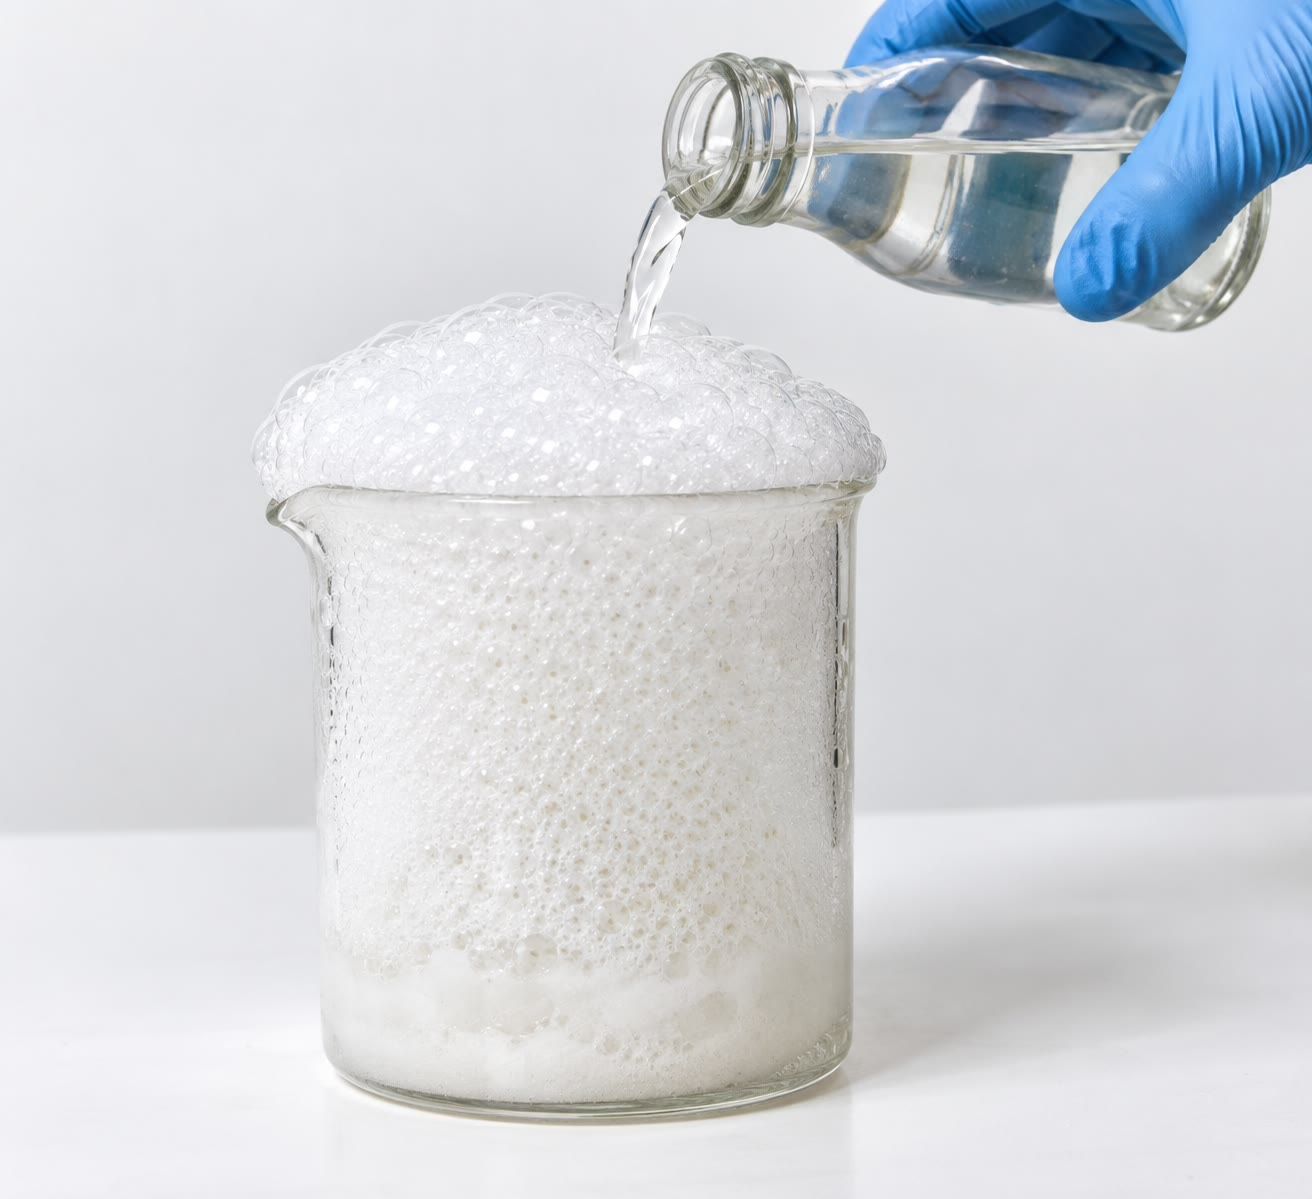
\includegraphics[width=0.5\linewidth]{images/book1/ai/g5-baking-soda-lab.jpg}

{\small Vinagre sobre bicarbonato: se desprende un gas.}
\end{omfigure}

\section{Cambios útiles y cambios perjudiciales}

\begin{proposition}[Cambios químicos a nuestro alrededor]\label{prop:g5:irreversible-changes:around}
Muchos \omterm{def:g5:irreversible-changes:chemical-change}{cambios químicos} son útiles: cocinar los alimentos, hornear el
pan, quemar gas para calentar una casa, el fraguado del yeso o del
cemento. Otros causan daños: el hierro que se oxida, los alimentos que
se estropean, la madera que se pudre. No podemos deshacerlos, pero sí
hacerlos más lentos:
\begin{itemize}
  \item los alimentos se conservan más tiempo en el frío de la nevera;
  \item la pintura o una película de aceite mantienen el \omterm{def:g4:air-a-mixture-of-gases:air}{aire} y el agua
        lejos del hierro;
  \item una manzana cortada rociada con zumo de limón se pone marrón más
        despacio.
\end{itemize}
\end{proposition}

\begin{omfigure}
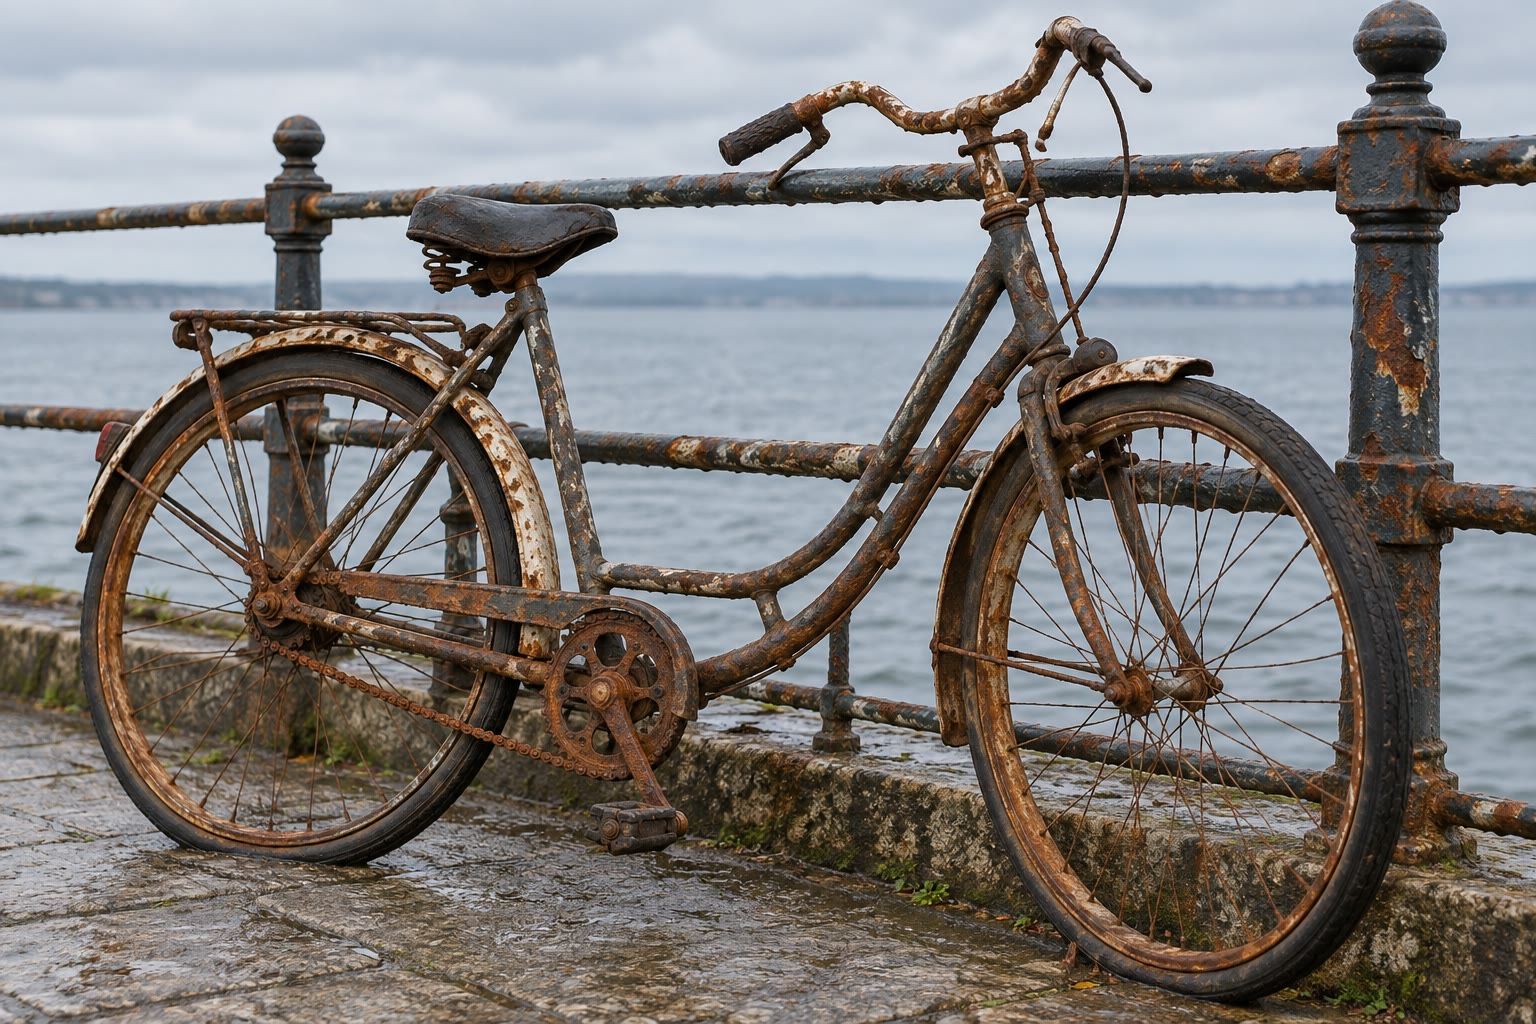
\includegraphics[width=0.55\linewidth]{images/book1/ai/g5-rusty-bicycle.jpg}

{\small Una bicicleta que ha pasado años bajo la lluvia: el hierro se ha
oxidado.}
\end{omfigure}

\begin{remark}[Deshacer, pero no sin más]\label{rem:g5:irreversible-changes:not-simply}
``No se puede deshacer'' significa que no hay un camino de vuelta
sencillo, como enfriar o secar. A veces los químicos consiguen
convertir la herrumbre otra vez en hierro, pero solo con un horno y con
sustancias nuevas: eso es otro \omterm{def:g5:irreversible-changes:chemical-change}{cambio químico}, no una vuelta atrás.
\end{remark}

\section{Ejercicios}

\begin{exercise}[$\star$]\label{exo:g5:irreversible-changes:1}
Di si cada cambio se puede deshacer: fundir chocolate, quemar una
cerilla, \omterm{def:g2:mixing-and-dissolving:dissolve}{disolver} sal en agua, tostar pan.
\end{exercise}

\begin{exercise}[$\star$]\label{exo:g5:irreversible-changes:2}
¿Qué es un \omterm{def:g5:irreversible-changes:chemical-change}{cambio químico}? Da dos ejemplos de la cocina.
\end{exercise}

\begin{exercise}[$\star$]\label{exo:g5:irreversible-changes:3}
Se \omterm{def:g2:mixing-and-dissolving:dissolve}{disuelve} sal en agua. ¿Cómo se puede recuperar la sal? ¿\omterm{def:g2:mixing-and-dissolving:dissolve}{Disolver} es
un \omterm{def:g5:irreversible-changes:reversible}{cambio reversible}?
\end{exercise}

\begin{exercise}[$\star$]\label{exo:g5:irreversible-changes:4}
¿Qué pistas de un \omterm{def:g5:irreversible-changes:chemical-change}{cambio químico} notas cuando la leche se agria? Da
dos.
\end{exercise}

\begin{exercise}[$\star$]\label{exo:g5:irreversible-changes:5}
Mira la figura de las dos columnas. ¿Qué cambios tienen una doble
flecha? ¿Qué significa la doble flecha?
\end{exercise}

\begin{exercise}[$\star$]\label{exo:g5:irreversible-changes:6}
¿Por qué se engrasa la cadena de una bicicleta? ¿Qué \omterm{def:g5:irreversible-changes:chemical-change}{cambio químico}
frena el aceite?
\end{exercise}

\begin{exercise}[$\star$]\label{exo:g5:irreversible-changes:7}
Cuando se vierte vinagre sobre bicarbonato, burbujea. ¿Qué pista es
esta?
\end{exercise}

\begin{exercise}[$\star$]\label{exo:g5:irreversible-changes:8}
Nombra un \omterm{def:g5:irreversible-changes:chemical-change}{cambio químico} útil y un \omterm{def:g5:irreversible-changes:chemical-change}{cambio químico} perjudicial.
\end{exercise}

\begin{exercise}[$\star$]\label{exo:g5:irreversible-changes:9}
¿Por qué guardamos la leche en la nevera?
\end{exercise}

\begin{exercise}[$\star\star$]\label{exo:g5:irreversible-changes:10}
El agua burbujea cuando hierve. ¿Hervir es un \omterm{def:g5:irreversible-changes:chemical-change}{cambio químico}? Explica
por qué no basta con una sola pista.
\end{exercise}

\begin{exercise}[$\star\star$]\label{exo:g5:irreversible-changes:11}
Tom dice: ``Cuando la vela \omterm{def:g4:what-a-fire-needs:burning}{arde}, la cera simplemente se derrite, como
el hielo''. Usa dos pistas para explicar por qué quemar una vela es un
\omterm{def:g5:irreversible-changes:chemical-change}{cambio químico}, y no solo una fusión.
\end{exercise}
